% \iffalse meta-comment
%
% Copyright (C) 2017--2020 by Xiangdong Zeng <xdzeng96@gmail.com>
%
% This work may be distributed and/or modified under the
% conditions of the LaTeX Project Public License, either
% version 1.3c of this license or (at your option) any later
% version. The latest version of this license is in:
%
%   http://www.latex-project.org/lppl.txt
%
% and version 1.3 or later is part of all distributions of
% LaTeX version 2005/12/01 or later.
%
% This work has the LPPL maintenance status `maintained'.
%
% The Current Maintainer of this work is Xiangdong Zeng.
%
% \fi

%*********************************************************************
% fduthesis: 复旦大学论文模板
% 2020/08/30 v0.7e + 2021/12/20 期末论文魔改版
%
% 重要提示:
%   1. 请确保使用 UTF-8 编码保存
%   2. 请使用 XeLaTeX 或 LuaLaTeX 编译
%   3. 请仔细阅读用户文档
%   4. 修改、使用、发布本文档请务必遵循 LaTeX Project Public License
%   5. 不需要的注释可以尽情删除
%*********************************************************************

%\documentclass{fduthesis}
% 模板选项:
%   type = doctor|master|bachelor  论文类型,默认为本科论文
%   oneside|twoside                论文的单双面模式,默认为 twoside
%   draft = true|false             是否开启草稿模式,默认关闭
% 带选项的用法示例:
%   \documentclass[oneside]{fduthesis}
%   \documentclass[twoside, draft=true]{fduthesis}
\documentclass[type=master, twoside, draft=false]{fduthesis}

\fdusetup{
  % 参数设置
  % 允许采用两种方式设置选项:
  %   1. style/... = ...
  %   2. style = { ... = ... }
  % 注意事项:
  %   1. 不要出现空行
  %   2. “=” 两侧的空格会被忽略
  %   3. “/” 两侧的空格不会被忽略
  %   4. 请使用英文逗号 “,” 分隔选项
  %
  % style 类用于设置论文格式
  style = {
    font = times,
    % 西文字体(包括数学字体)
    % 允许选项:
    %   font = garamond|libertinus|lm|palatino|times|times*|none
    %
    cjk-font = fandol,
    % cjk-font = windows,
    % 中文字体
    % 允许选项:
    %   cjk-font = adobe|fandol|founder|mac|sinotype|sourcehan|windows|none
    %
    % 注意:
    %   1. 中文字体设置高度依赖于系统。各系统建议方案:
    %        windows:cjk-font = windows
    %        mac:    cjk-font = mac
    %        linux:  cjk-font = fandol(默认值)
    %   2. 除 fandol 和 sourcehan 外,其余字体均为商用字体,请注意版权问题
    %   3. 但 fandol 字体缺字比较严重,而 sourcehan 没有配备楷体和仿宋体
    %   4. 这里中西文字体设置均注释掉了,即使用默认设置:
    %        font     = times
    %        cjk-font = fandol
    %   5. 使用 font = none / cjk-font = none 关闭默认字体设置,需手动进行配置
    %
    font-size = -4,
    % 字号
    % 允许选项:
    %   font-size = -4|5
    %
    % fullwidth-stop = catcode,
    % 是否把全角实心句点 “.” 作为默认的句号形状
    % 允许选项:
    %   fullwidth-stop = catcode|mapping|false
    % 说明:
    %   catcode   显式的 “。” 会被替换为 “.”(e.g. 不包括用宏定义保存的 “。”)
    %   mapping   所有的 “。” 会被替换为 “.”(使用 LuaLaTeX 编译则无效)
    %   false     不进行替换
    %
    footnote-style = xits,
    % 脚注编号样式
    % 允许选项:
    %   footnote-style = plain|libertinus|libertinus*|libertinus-sans|
    %                    pifont|pifont*|pifont-sans|pifont-sans*|
    %                    xits|xits-sans|xits-sans*
    %
    % hyperlink = color,
    % 超链接样式
    % 允许选项:
    %   hyperlink = border|color|none
    %
    % hyperlink-color = default,
    % 超链接颜色
    % 允许选项:
    %   hyperlink-color = default|classic|elegant|fantasy|material|
    %                     business|science|summer|autumn|graylevel|prl
    % 默认与西文字体保持一致
    %
    bib-backend = bibtex,
    % 参考文献支持方式
    % 允许选项:
    %   bib-backend = bibtex|biblatex
    %
    % bib-style = numerical,
    % 参考文献样式
    % 允许选项:
    %   bib-style = author-year|numerical|<其他样式>
    % 说明:
    %   author-year  著者—出版年制
    %   numerical    顺序编码制
    %   <其他样式>   使用其他 .bst(bibtex)或 .bbx(biblatex)格式文件
    %
    % cite-style = {},
    % 引用样式
    % 默认为空,即与参考文献样式保持一致
    % 仅适用于 biblatex;如要填写,需保证相应的 .cbx 格式文件能被调用
    %
    bib-resource = {cite,papers},
    % 参考文献数据源
    % 可以是单个文件,也可以是用英文逗号 “,” 隔开的一组文件
    % 如果使用 biblatex,则必须明确给出 .bib 后缀名
    %
    % logo = {fudan-name.pdf},
    % 封面中的校名图片
    % 模版已自带,通常不需要额外配置
    %
    % logo-size = {0.5\textwidth},      % 只设置宽度
    % logo-size = {{}, 3cm},            % 只设置高度
    % logo-size = {8cm, 3cm},           % 设置宽度和高度
    % 设置校名图片的大小
    % 通常不需要调整
    %
    % auto-make-cover = true
    % 是否自动生成论文封面(封一)、指导小组成员名单(封二)和声明页(封三)
    % 除非特殊需要(e.g. 不要封面),否则不建议设为 false
  },
  %
  % info 类用于录入论文信息
  info = {
    title = {持续集成和持续部署平台及实践体会},
    % 中文标题
    % 长标题建议使用 “\\” 命令手动换行(不是指在源文件里输入回车符,当然
    % 源文件里适当的换行可以有助于代码清晰):
    %   title = {最高人民法院、最高人民检察院关于适用\\
    %            犯罪嫌疑人、被告人逃匿、死亡案件违法所得\\
    %            没收程序若干问题的规定},
    %
    title* = {},
    % 英文标题
    %
    author = {蒋骐泽},
    % 作者姓名
    %
    student-id = {21110240072},
    % 作者学号
    %
    major = {软件过程管理},
    % 课程名称
    %
    student-id = {21110240072},
    % 作者学号
    %
    date = {2022 年 6 月 27 日},
    % 日期
    % 注释掉表示使用编译日期
    %
  }
}

% 需要的宏包可以自行调用
%\usepackage{physics}
\usepackage{comment}
\usepackage{color}
\usepackage[ruled,noend]{algorithm2e}
\SetAlgorithmName{算法}{algorithmautorefname}{}
\usepackage{multirow}
\usepackage[figuresright]{rotating}
\usepackage{listings}
\usepackage{lscape}
\usepackage{graphicx}

% 需要的命令可以自行定义
%\newcommand{\hilbertH}{\symcal{H}}
%\newcommand{\ee}{\symrm{e}}
%\newcommand{\ii}{\symrm{i}}
\newcommand{\qize}[1]{{\color{red} {\textbf{#1}}}}

\newtheorem{problem}{问题}
\newtheorem{proposition}{命题}
\newtheorem{assumption}{假设}

\begin{document}

% 这个命令用来关闭版心底部强制对齐,可以减少不必要的 underfull \vbox 提示,但会影响排版效果
% \raggedbottom

% 前置部分包含目录、中英文摘要以及符号表等
\frontmatter

% 目录
\tableofcontents
% 插图目录
%\listoffigures
% 表格目录
% \listoftables


\begin{abstract}
  
  在软件开发过程中,持续集成和持续部署的重要性越发凸显,在大型项目中,是必备的技术之一。
  通过持续集成,软件开发可以有更高的效率,能够快速发现代码问题,并在提高代码上线的速度。
  本文对持续集成和持续部署两个概念进行介绍,同时列举了几个目前较为流行的持续集成和
  持续部署平台并介绍其功能。最后,基于本次课程项目,对项目中所涉及的框架及代码进行介绍,
  并总结了项目开发中碰到的困难和体会。
  
  注:本人负责前端部分编写,但是由于其他组员未完成其他部分代码编写,最后本人独立完成了
  API设计,前端、后端、测试代码编写,以及代码的持续集成、持续部署相关配置。
  

\end{abstract}


% 符号表
% 语法与 LaTeX 表格一致:列用 & 区分,行用 \\ 区分
% 如需修改格式,可以使用可选参数:
%   \begin{notation}[ll]
%     $x$ & 坐标 \\
%     $p$ & 动量
%   \end{notation}
% 可选参数与 LaTeX 标准表格的列格式说明语法一致
% 这里的 “ll” 表示两列均为自动宽度,并且左对齐
%\begin{notation}[ll]
%  $x$                  & 坐标        \\
%  $p$                  & 动量        \\
%  $\psi(x)$            & 波函数      \\
%  $\bra{x}$            & 左矢(bra) \\
%  $\ket{x}$            & 右矢(ket) \\
%  $\ip{\alpha}{\beta}$ & 内积        \\
%\end{notation}

% 主体部分是论文的核心
\mainmatter

% 建议采用多文件编译的方式
% 比较好的做法是把每一章放进一个单独的 tex 文件里,并在这里用 \include 导入,例如
%   \include{chapter1}
%   \include{chapter2}
%   \include{chapter3}


\chapter{引言}\label{chap:introduction}

随着软件规模越来越大,同时开发效率和开发周期要求变高,传统的软件开发、测试、部署流程已经难以适应当前的开发需求。
如果仍然依靠手动编译、测试和部署,将会大大降低开发的效率。例如一个包含前端、后端、数据库等模块的系统,
当其中一个模块修改后,需要测试各个不同模块都能够正常工作,需要编译部署所有相关模块并执行各自的测试用例,
在通过测试后将模块上线部署。这一系列工作涉及不同环境,步骤复杂,因此很有必要引入自动化,
在代码进行提交和合并的时候自动进行,从而提升代码部署效率,同时能够更快的发现和定位问题,减少上线事故。

在软件开发实践中,对代码自动编译、测试和发布称为持续集成,而将通过集成的代码自动上线部署称为持续部署。
下面两节会对这两个方向的概念和涉及的部分技术细节进行介绍。

\section{持续集成}

持续集成(Continuous Integration, CI)是一种软件开发实践,当开发人员将代码合并至主分支时,持续集成系统会自动
根据最新合并代码,对项目进行构建并进行测试。使用持续集成,可以避免大家联合开发时,由于代码冲突或者对代码的
非预期修改导致代码合并后功能出错。同时,也可以让开发人员从繁重复杂的代码编译和测试中解放出来,
提升代码开发效率和稳定性。

使用持续集成,需要在进行软件开发时满足一定的条件。一般来说具有下述要求:

\subsection{使用代码版本控制系统}

在协同开发中,为了能够方便的进行代码合并和同步,对代码进行版本控制几乎是必不可少的。目前最流行的版本控制工具
是Git。在持续集成中,版本控制工具也是必须工具之一。对代码进行版本控制,可以选择进行持续集成的条件,
如仅对主分支的合并和提交进行持续集成,或是仅对代码标签进行持续集成,这样避免了对开发中的代码进行不必要的持续集成操作,
从而减少持续集成的资源消耗,同时也可以减少无意义的持续集成错误提示。

\subsection{完善的单元测试用例}

为了最大限度的发挥持续集成的优势,完善的单元测试是必不可少的。通过单元测试,持续集成时可以确认对代码的修改与之前
实现的功能没有冲突。同时,通过检查单元测试下代码的覆盖率,也可以发现单元测试的漏洞,提升测试有效性。
虽然仅靠单元测试不能发现所有代码非预期执行的问题,但是已经可以高效找到大部分显著的问题,避免了代码上线后
在生产环境出错所造成的的影响。

\subsection{持续集成服务器}
显然,由于持续集成时需要编译构建项目和运行测试代码,一台用于持续集成的服务器是必不可少的。
目前很多代码托管平台和云平台提供了持续集成的服务,不少平台的服务面向开源代码或是小规模团体是免费的。
服务器会持续监控被托管的代码,当代码满足集成触发要求时自动进行项目构建、测试和产物打包。

\section{持续部署}

持续部署(Continuous Deployment, CD)是在代码通过持续集成后将代码自动部署至生产环境,减少人工成本,提升部署效率的过程。
将代码部署到生产环境需要不小的工作量,尤其是一些大型分布式软件、或者是涉及多种运行环境不同的组件,
人工部署步骤繁杂,耗时且容易出现失误。通过持续部署,开发人员可以自动将新开发的软件部署到生产环境,
同时还可以支持特定的部署规则,例如灰度部署、自动回滚等,可以显著减轻运维的成本。

由于容器技术具有环境统一互不干扰、占用资源小、体积小、迁移扩展方便等显著优点,使用容器部署成为了目前线上任务的
主流方式之一。正由于容器有上述优点,在使用持续部署的过程中使用容器也是最合适的方式之一。同时,
Kubernetes(k8s)作为新兴的大规模容器编排技术,在大规模管理和部署容器上具有明显优势,
成为目前业界的主流。

由于持续部署一般涉及大型商用软件,同时普通用户一般没有很强的持续部署需求,所以相比持续集成,
提供持续部署服务的不是很多,同时功能比较简单。简单的持续部署功能在大部分开发套件中能够找到,
可以实现简单的持续部署。

\section{持续集成和持续部署平台}

目前有很多提供持续集成和持续部署的平台,它们各有特色。本文会针对接触过的三个持续集成部署平台AppVeyor、GitHub Actions和
华为云进行介绍。同时,基于本次课程实践,本文对本次课程实践中代码编写,持续集成和持续部署部分进行介绍,
也对其中遇到的困难和体会进行总结。
\chapter{AppVeyor}

AppVeyor是一个由加拿大成立于2011年的持续集成项目,并于2013年提供公开服务。
该平台最初的目标面向Windows项目,是早年免费为开源项目提供Windows持续集成服务的项目之一。

由于AppVeyor可以追踪GitHub中的提交,并对开源项目免费提供单线程的持续集成,
是很多开源项目选择的持续集成工具之一。通过AppVeyor,可以很方便的获取项目产出文件,
同时在合并分支前对代码兼容性进行初步检查,发现无法通过编译的合并请求。

使用AppVeyor,首先需要创建新项目。可以看到,AppVeyor支持几乎所有的主流的基于Git的代码管理平台,
包括使用Git协议的私人平台,因此很容易集成。选择项目后,AppVeyor会监控该项目,并在满足集成条件时
使用项目最新的代码进行集成,并给出项目产物,免去了开发人员和使用者需要手动编译的麻烦。

\begin{figure}[h]
    \centering
    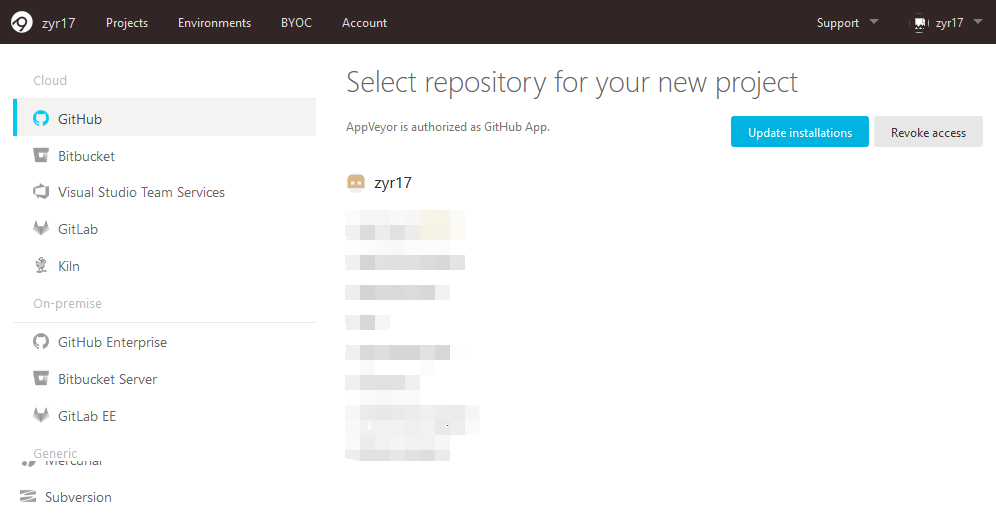
\includegraphics[width=1\textwidth]{figures/appveyor/create.png}
    \caption{创建新AppVeyor项目}
    \label{fig:appveyor_create}
\end{figure}

最方便的使用AppVeyor的方法是在项目中添加appveyor.yml,AppVeyor会自动读取该文件并根据文件中的
配置和命令进行自动集成。我们也可以手动对项目进行设置,例如指定其他名称的配置文件,
或者将配置文件写于AppVeyor上而非读取代码库中的配置文件。

以某个项目的配置文件为例,本文会对AppVeyor的项目配置做简要介绍。

\begin{figure}[h]
    \centering
    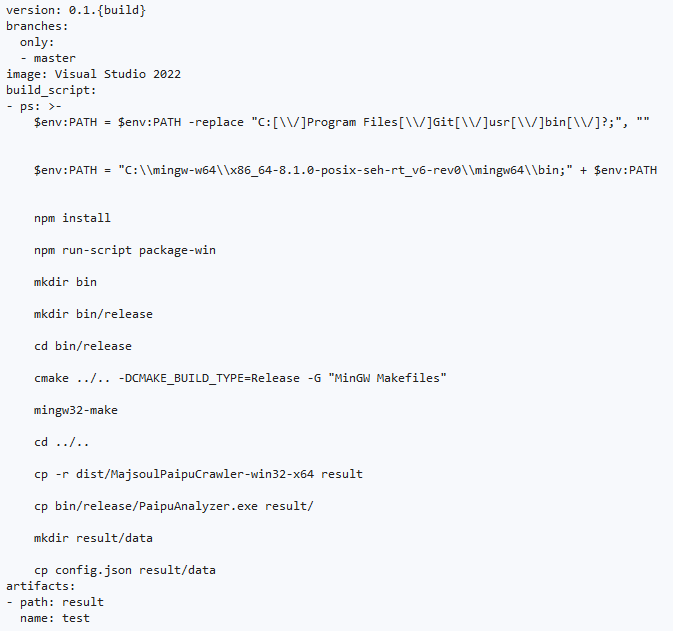
\includegraphics[width=1\textwidth]{figures/appveyor/config.png}
    \caption{AppVeyor配置文件}
    \label{fig:my_label}
\end{figure}

首先配置中需要指定每次集成的版本号。由于需要保证每次的版本号不一样,所以包含一个
每次集成后自增1的build。然后需要指定在什么情况下触发自动集成,这里的设置是
仅当master分支有新的commit时触发。接下来是指定运行环境,这里的Visual Studio 2022
并非单指该IDE,而代表了以Visual Studio为主的一系列环境。显然,这是一个Windows环境,
用于编译Windows项目,AppVeyor目前也提供Linux和Mac项目的持续集成服务。在build\_script
中,是集成时需要执行的命令。在该配置中,使用了PowerShell作为集成命令行。同时,
AppVeyor对脚本的设置类似markdown,除非连续两个换行符,否则将多行脚本看成单行脚本,
这样便于在配置中编写较长的脚本,但也会增加多行脚本的行数。最后,在持续集成完成后,
使用artifacts指定产物目录和文件名,这样就能够在验证代码有效性的同时直接获取构建产物。

AppVeyor作为早期平台,其易用性较高,但是支持较为单一,由于底层基于虚拟机实现,
工作流类似于在一台服务器上进行编译,较难实现复杂的控制流和多任务,
目前在开源社区用于用于自动构建产物较多。
\chapter{GitHub Actions}

GitHub Actions是由著名代码托管平台GitHub推出的持续集成和持续部署工具,
于2020年提供于所有GitHub用户使用。除了开源代码库可以免费使用该功能外,
还为每个账户提供了每月多达2000分钟的私有仓库运行时间。同时,
GitHub Actions还同时支持Windows、Linux、MacOS环境,提供流水线功能,
支持并发集成和测试,快速引用其他人编写的集成工具等,是一个功能强大的工具。

GitHub Actions目前只支持托管于GitHub上的仓库使用。一个仓库使用GitHub
Actions需要在.github/workflows/中新建定义一个Action的yml文件,
一个仓库可以有多个Action文件,用于不同任务。

\begin{figure}
    \centering
    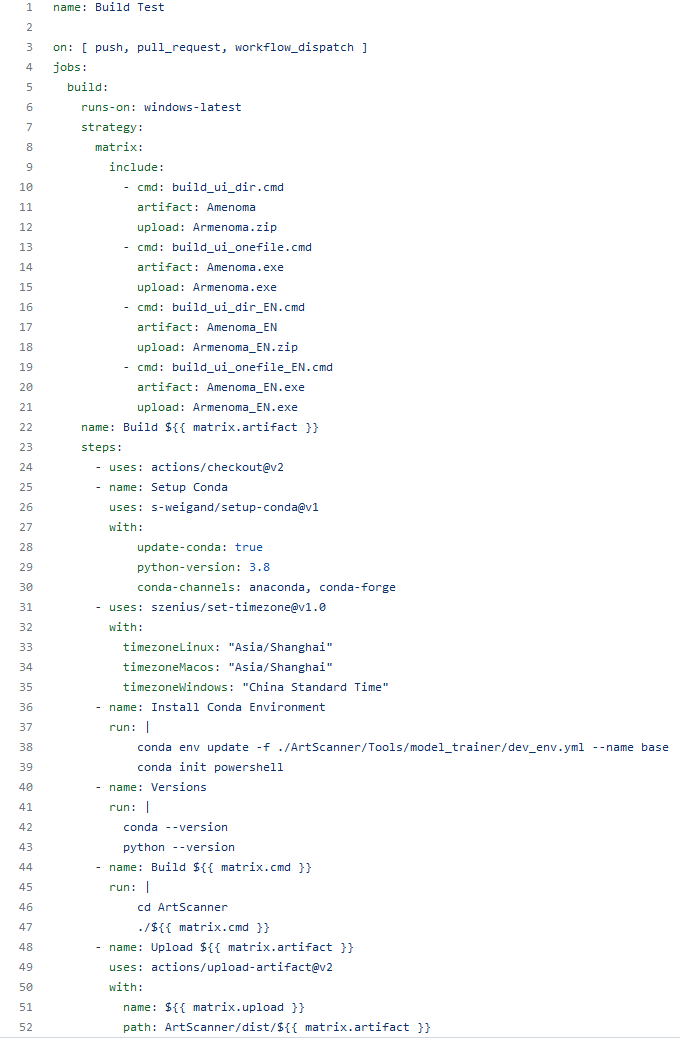
\includegraphics[width=1\textwidth]{figures/github/actions.png}
    \caption{GitHub Actions}
    \label{fig:githubactions}
\end{figure}

图\ref{fig:githubactions}给出了一份GitHub Actions配置。

第1行定义了工作流的名称,第3行定义了工作流的触发条件。接下来定义了不同的jobs,
本例中只包含一个build的job,在一些大型项目中,可以包含编译、测试、打包等不同的job,
且不同的job之间可以进行文件传递,且可以指定依赖关系,因此可以完成交叉编译等复杂任务。

第7-21行是GitHub Actions的策略矩阵功能,可以同时启动多个实例执行较为相似的任务。
在本例中,由于产物包含中文、英文、可执行文件和压缩包共四种组合产物,其持续集成代码接近,
通过策略矩阵,可以同时编译四种产物,大大减少编译时间的同时还减轻了工作流编写的代码量。
策略矩阵也被常用于同时执行大量单元测试。

在第24、26、31、49行,引用了其他人编写的配置,这是GitHub Actions的一个特色,
这些配置均为GitHub中的一个仓库,这种方式大大提高了Actions的灵活性和可复用性。
在本例中,引用的配置分别用于自动从GitHub拉取代码,激活conda环境,设置时区,
以及上传集成后产物。

第37-47行为执行脚本,GitHub Actions基于容器实现,在执行时内部环境和普通服务器无异,
因此可以很方便的进行复杂配置。

在本例中配置并未包含流水线和持续部署相关的代码,实际上GitHub Actions均可以实现。
对于流水线,只需要启动多个jobs,例如build/test/deploy并指定依赖关系,
就可以做到流水线作业。而对于持续部署,GitHub仓库中可以设定Actions执行时
可以使用的隐私信息,通过将SSH私钥或服务器密码等设置为隐私信息,
服务器可以在持续集成完成后通过密钥访问部署服务器并进行自动部署。
然而,作为一个提供公开服务且位于国外的公司,这样做的安全性较低,
仅作为小规模、低成本、个人服务器部署的可选方案,例如利用Actions对静态网页自动
编译,并将编译结果上传至博客服务器等。
\chapter{华为云DevCloud}

本次课程作业在华为云DevCloud上完成,华为云在上面一站式提供了项目规划、代码管理、
持续集成、持续部署、文档编写等功能,涉及项目开发的几乎所有方面。
本文对其持续集成和持续部署方面进行介绍和总结。

在华为云的构建\&发布中,共涉及流水线、编译构建、部署、发布和运维五部分。
本次课程作业中主要涉及了前三部分,发布和运维暂无涉及。

\begin{figure}[h]
    \centering
    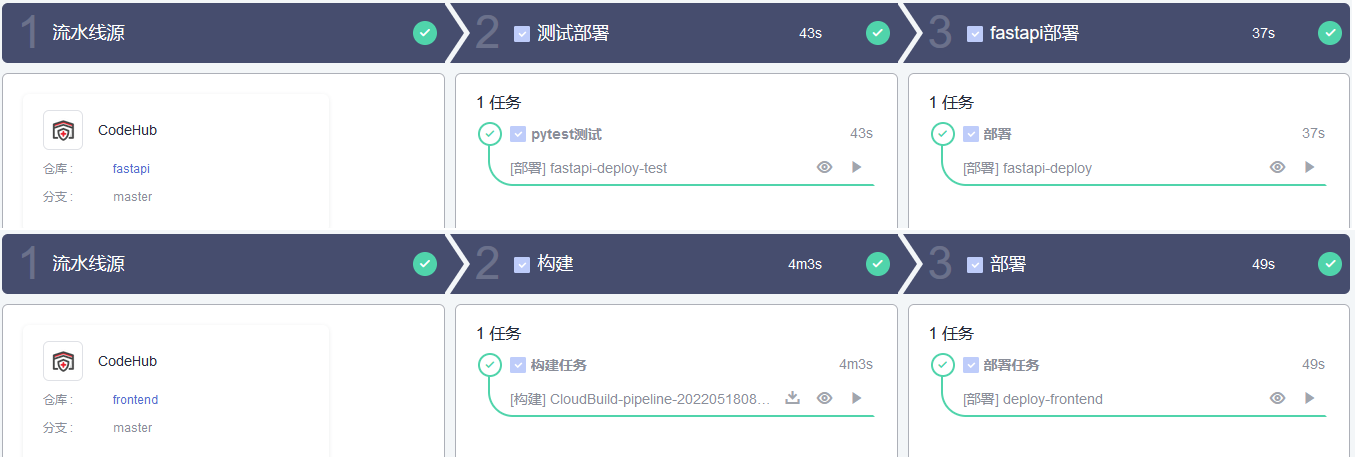
\includegraphics[width=1\textwidth]{figures/huawei/pipeline.png}
    \caption{华为云流水线}
    \label{fig:huawei_pipeline}
\end{figure}

在图\ref{fig:huawei_pipeline}中,展示了两条前端流水线。流水线会绑定一个代码仓库,
当满足触发条件后按顺序执行流水线上的操作。操作有多种,
本例中前端的流水线为构建镜像并部署,后端的流水线为先进行测试部署再进行部署。
当前阶段出现错误后,流水线默认会自动停止执行。
以后端为例,如果某次代码变动导致代码未通过测试部署,那么将会停止流水线,
从而避免错误代码直接部署上线。

\begin{figure}[h]
    \centering
    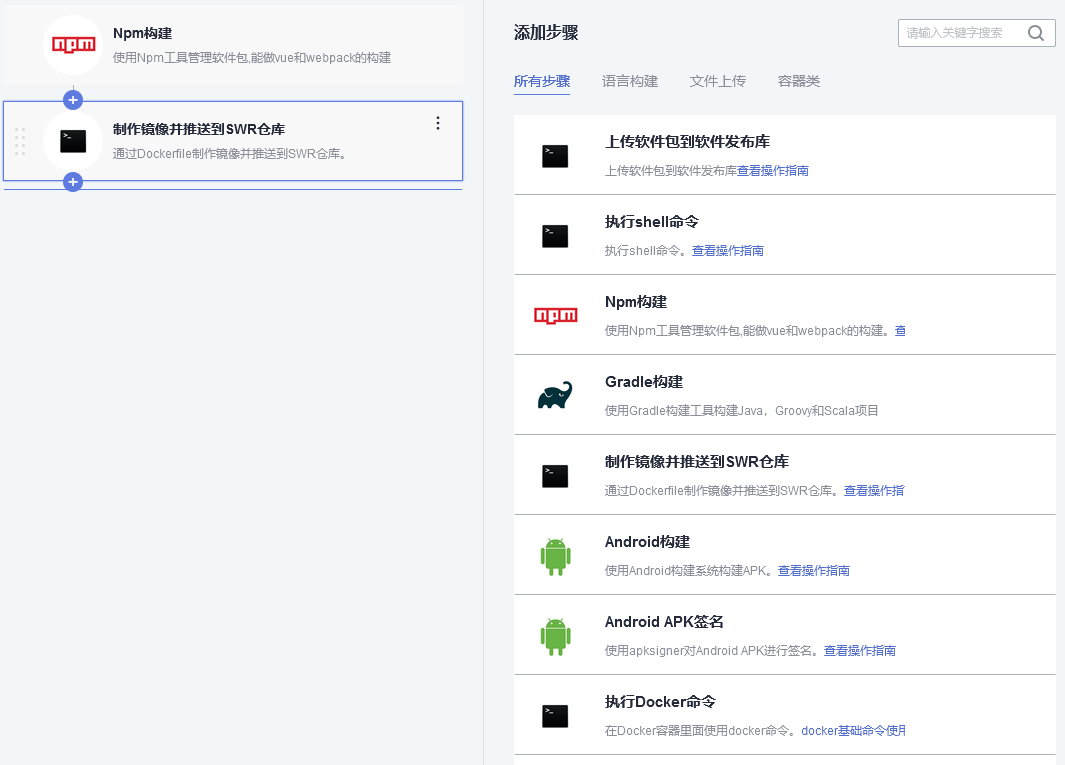
\includegraphics[width=1\textwidth]{figures/huawei/build.png}
    \caption{华为云编译和构建}
    \label{fig:huawei_build}
\end{figure}

流水线每个阶段执行的任务在编译构建和部署中事先创建,并在流水线中被引用。
相比AppVeyor和GitHub Actions中需要自己编写配置文件,图\ref{fig:huawei_build}中看到
华为云以可视化的方式提供了丰富的步骤, 让开发人员不用手动编写构建或者部署代码。

相比其他重点在持续集成的平台,由于华为云自己就提供云主机的服务,
因此提供了主机组管理的功能。华为云支持将多台主机指定为一个主机组,
部署时可以针对整个主机组一次性全部部署,降低了部署工作量。
\chapter{基于华为云的课程实践}

本次课程项目基于华为云,需要完成一个自习室预定系统,
并利用华为云进行代码管理、持续集成和持续部署。
本文对本人编写的API设计,前端、后端、测试代码及华为云持续集成和持续部署模块进行介绍。

\section{项目框架}

项目分为前端和后端,前端使用Web技术栈,并通过Web API和后端进行通信。
后端使用RESTful风格设计通信接口,在服务器监听API请求,并与数据库通信进行信息的获取和存储。
同时,编写后端代码时同时编写相关单元测试用例,用于检查代码编写的正确性。

\section{代码构成}

\subsection{API设计}

\begin{figure}
    \centering
    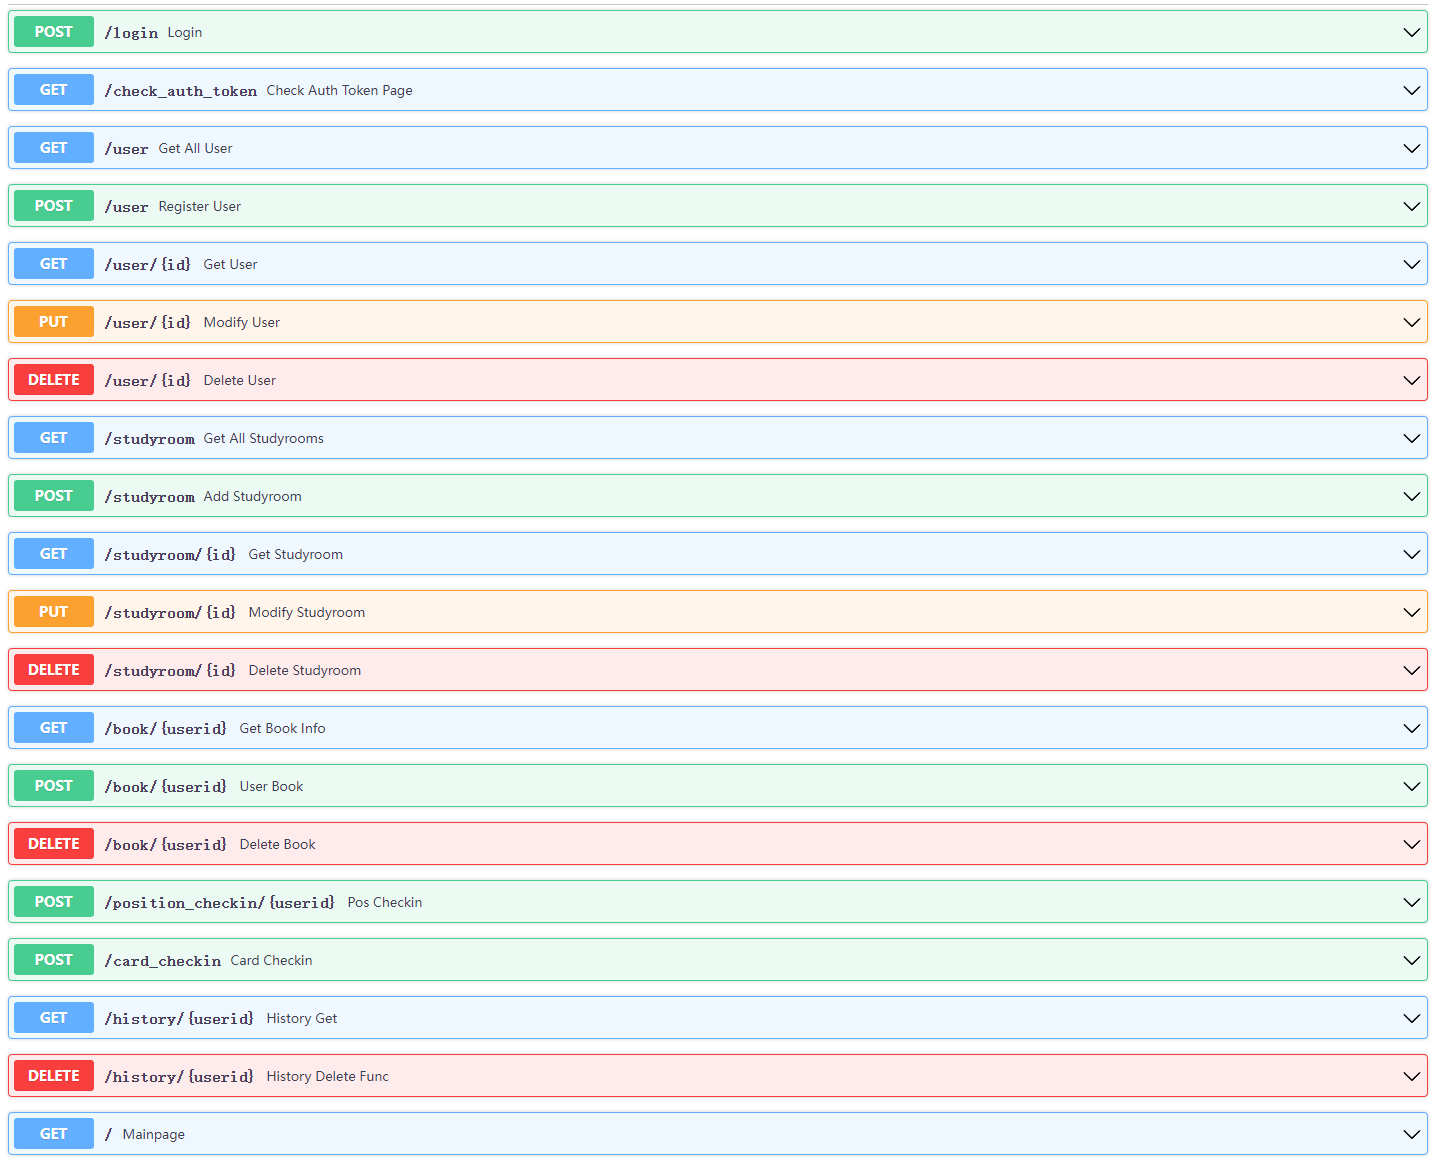
\includegraphics[width=\textwidth]{figures/project/API.png}
    \caption{通信API}
    \label{fig:project_api}
\end{figure}

如图\ref{fig:project_api}所示,项目使用RESTful思想设计API。除去用户注册和用户登录,其他API请求均需要携带Auth-Token标头
提供认证token,后端以此验证身份。API分为账户管理、自习室管理、预约管理、签到管理、历史管理五类,
可在后端代码介绍中看到。

\subsubsection{前端代码}

前端代码基于Vue 2.0框架,基于助教提供的脚手架。框架中以App.vue作为主页面,
包含了导航栏和通知模块,使用Vue Router功能完成非刷新的页间跳转。
图\ref{fig:project_admin_login}展示了管理员登录后的用户管理页面。

\begin{figure}
    \centering
    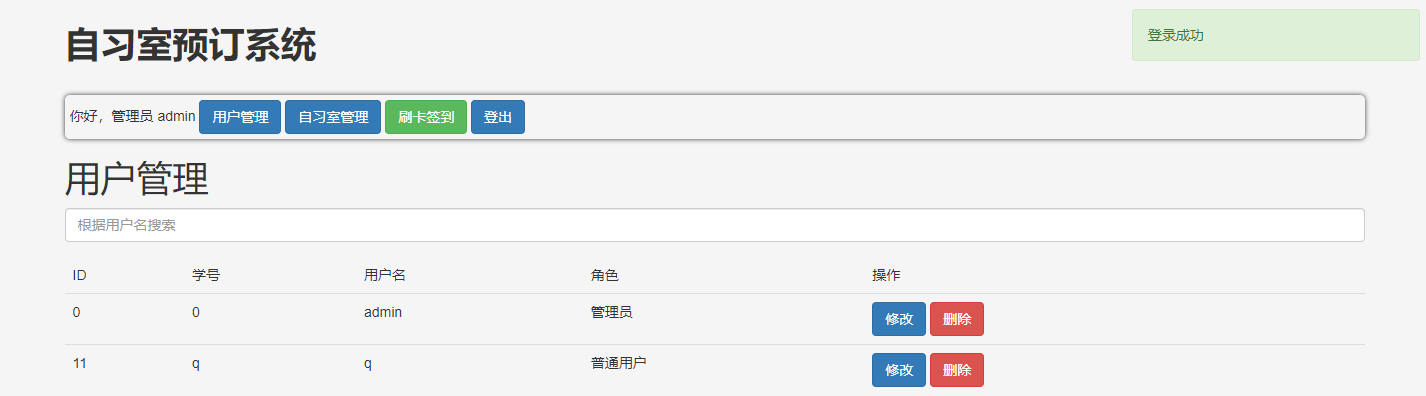
\includegraphics[width=\textwidth]{figures/project/frontend_admin_login.png}
    \caption{前端管理员账户登录页面}
    \label{fig:project_admin_login}
\end{figure}

其中导航栏根据当前的登录状态和不同用户身份会展示不同的功能按钮。
未登录时展示注册和登录按钮;普通用户登录后展示个人信息、签到、预约、历史、登出按钮;
管理员登录后展示用户管理、自习室管理、刷卡签到、登出按钮。

前端需要持久化维护的信息只有用户认证token、用户身份、用户ID和token过期时间,
这些信息会存于Vue Store和localStorage中。当首次加载页面发现token已经过期时,
前端会自动清除已有信息并返回登录页面。由于后端同样会对用户token及信息做验证,
因此在前端伪造持久化信息除了能够展示页面外没有办法获取数据。

页面间进行信息传递使用Vue Store。除了上述身份和认证信息外,仅提示信息(右上角成功提示)
需要传递,主页面加载提示框控件后,控件绑定store中提醒内容,当收到提醒后会自动渲染
最近5秒内的提醒。其他信息均在访问时向后端请求,减少信息泄漏。

\subsection{后端代码}

\begin{figure}
    \centering
    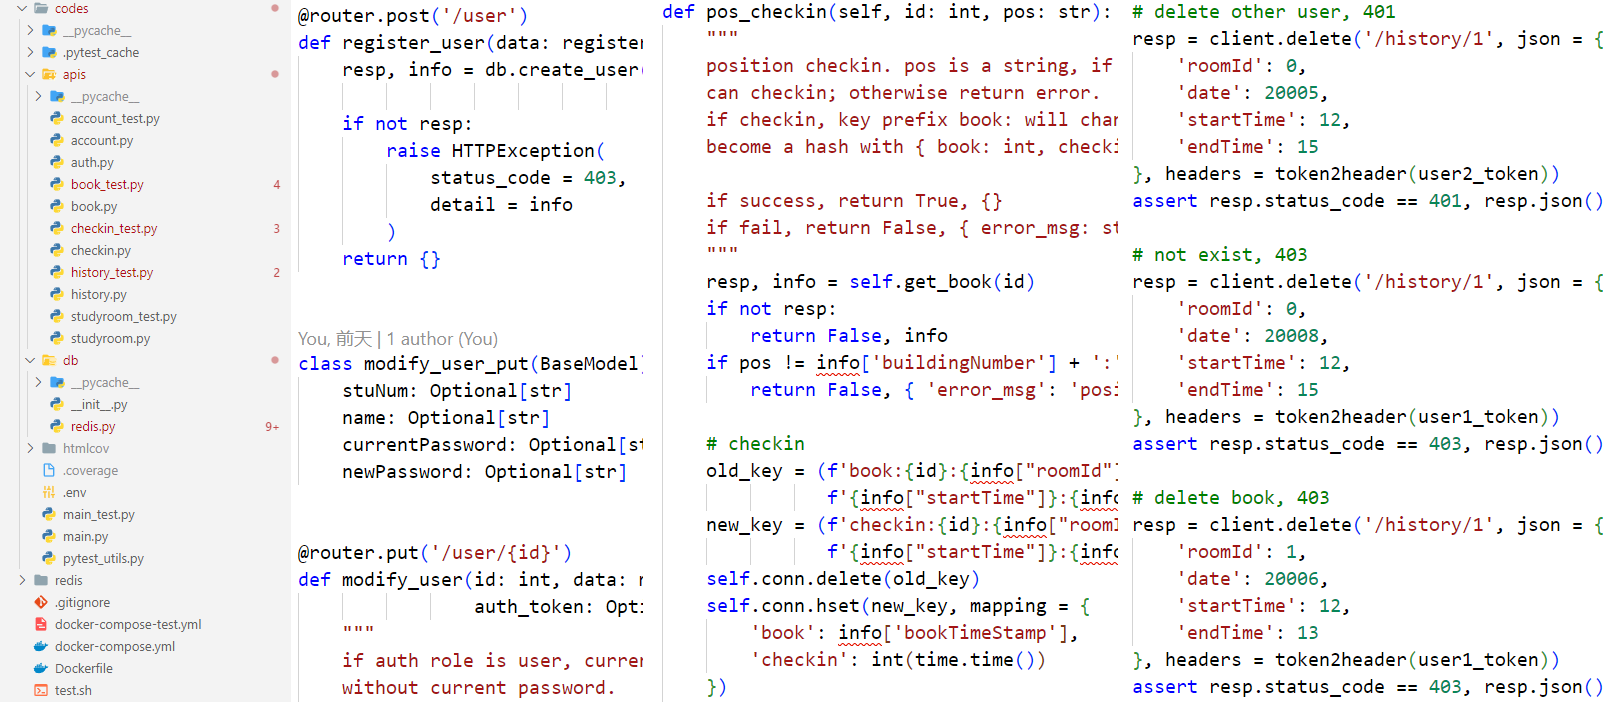
\includegraphics[width=\textwidth]{figures/project/backend_code.png}
    \caption{后端代码结构,及后端,数据库和测试代码片段}
    \label{fig:project_backend_code}
\end{figure}

\begin{figure}
    \centering
    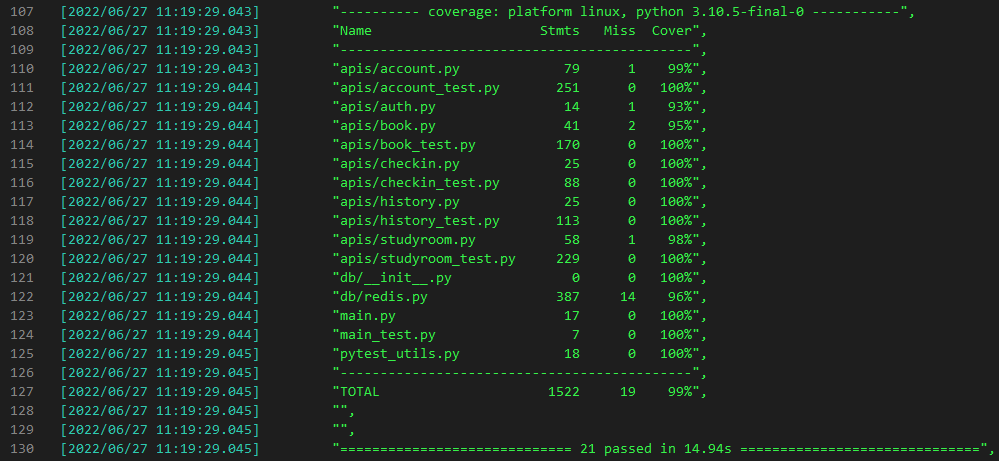
\includegraphics[width=\textwidth]{figures/project/coverage.png}
    \caption{后端代码coverage测试结果}
    \label{fig:project_coverage}
\end{figure}

图中展示了后端代码的结构,以及从左往右分别为后端、数据库操作和测试的部分代码片段。
后端代码使用Python FastAPI框架,并使用PyTest编写单元测试,coverage检查代码覆盖率。
根据API设计中所提到的,将API分为五大类,每类包含一个文件。同时,对每个文件编写了
一个单元测试文件,包含若干测试用例,测试基于API,检查返回值和返回数据是否正确。
同时,coverage也会检查代码的覆盖率,用于观察是否有代码漏写测试用例。
图\ref{fig:project_coverage}中展示了一次持续集成中coverage的代码覆盖率,其中未覆盖代码均为函数调用时一些异常情况的冗余判断,
由于之前调用函数时已经包含相关判断,因此该判断永远不成立。其余逻辑代码均实现了测试的全覆盖。

数据库部分,目前使用了轻量级数据库redis。由于使用类进行数据库操作,
因此写在了一个文件中。设计时准备将数据库类设计为单类,
但由于分析后发现当前数据库非单类也能正常工作,就未实现单类模式。

由于使用类包装了数据库访问接口,因此后端不关心数据库的实际实现,
只要接口保持一致,可以很方便的切换为其他数据库。
同时,当前数据库未根据API分类进行拆分,且和后端代码耦合。实际中可以将后端独立出来,
作为另一个服务,后端通过服务接口访问数据库,这样可以更加降低耦合度。
如果将数据库相关代码剥离,由于各类API之间互不关联,该后端代码也可以很容易的改造为微服务架构。

Redis作为轻量级键值对数据库,具有很高的吞吐性能,一般作为内存数据库和缓存数据库使用。
在本项目中,由于需要存储的数据种类较少,且相互依赖关系较为简单(仅预定座位时,预定操作
会依赖于用户和自习室),为了开发简便,未使用关系型数据库。实际项目中,
对于有较为复杂的依赖关系的情形,使用关系型数据库可以减少依赖关系出错的情况。

\section{华为云持续集成和持续部署}

由于前端和后端分别为两个代码仓库,采用了两条CI+CD流水线,
如图\ref{fig:huawei_pipeline}所示。由于Docker部署的简便性,前端和后端均使用Docker
进行部署,其中后端的Python和数据库环境分离,由两个container构成,使用docker-compose统一部署
和通信,并仅暴露FastAPI的接口可供外部访问,因此内部redis数据库无需进行身份验证,
减少工作量。

在前端代码的CI+CD中,首先会利用华为云的编译构建功能,使用NodeJS构建前端代码。
然后基于Nginx镜像,将编译完成后的代码复制到镜像中,同时编写Nginx配置,
将编译完成的静态网页配置访问。之后,将该镜像打包上传至华为云的镜像管理,
用于之后部署。在部署阶段,华为云会通过主机组的SSH访问本组使用的服务器,
停止当前运行的容器,拉取最新版本的镜像,并使用最新镜像重新启动容器。

在后端代码的CI+CD中,由于华为云的构建和测试功能不够定制化,
使用测试部署的方式进行。由于基于docker-compose的方式,进行测试部署非常容易。
同时只需在测试时将启动FastAPI换为执行pytest,测试时不会暴露接口,数据库也新启动一个
独立数据库, 在同一台服务器上执行测试完全不会影响
该服务器上已运行的线上服务。这更加体现了使用容器技术的优越性。
后端代码提交后会先进行测试部署,此时会使用pytest检查后端代码是否能够通过
所有测试用例,并给出代码覆盖率的报告。如果代码通过了测试,
则会进行代码部署,通过SSH连接服务器,停止当前运行的docker,拉取最近代码,
重新构建镜像并启动新实例。

经过上述流水线的配置,对于前端和后端代码,仅需要直接推送代码至代码库,
流水线就会自动对代码进行持续集成,并在通过编译和测试后自动部署到服务器上,全程
不需要人工干预。在持续集成失败后对线上服务不会造成影响,在持续集成通过后
线上服务仅会在停止并重新启动实例时断线不到10秒,并在之后无缝升级。

\section{实践中遇到的困难和体会}

在使用华为云进行CI和CD时,也碰到了很多困难。本节中会对碰到的一些困难和体会进行总结。

\subsection{权限和认证问题}

该问题出现在流水线阶段。首先是流水线由本人搭建,因此测试时没有发现流水线有执行权限的问题。
虽然将流水线设置为了任意用户均可执行,但是其中涉及到镜像的推送,由于推送到的镜像
仓库的owner是我自己,因此我可以直接推送,而别人不行。虽然之后修改了推送权限,
但是由于组员都不开发了所以未测试是否修改成功。

另一个认证问题则来自于认证Token。华为云中通过填写认证Token对镜像进行推送认证,
然而在示例代码中Token的时效只有24小时。这导致了最开始可以执行的流水线一天以后
推送失败。解决方法是重新生成一个有效期是永久的Token。华为云在这里做的很不便利,
需要手动用华为云的CLI创建生成永久期限Token。

\subsection{Compose的测试和部署}

华为云的流水线套件中没有直接支持docker-compose的多容器部署的操作,
由于后端和数据库是两个容器,测试了很多种方式最后都失败了,
最后选择了直接测试部署到服务器上的方式完成CI流水线。相比而言
GitHub Actions中可进行的操作更多,环境更完整,这个方面华为云需要改进。

\subsection{Podman和Docker}

在提供的华为云服务器中,使用了Podman代替了Docker。一般情况下不会有问题,
但是在使用compose部署时仍然碰到了一些麻烦,最后通过在服务器上保存两份后端代码,
一份用于生产环境部署,一份用于测试部署解决该问题。当然,在实际情况下,不需要
在同一台服务器上共享,不会碰到类似问题。

\subsection{前端的本地调试}

前端需要搭配后端才能使用,目前的前端使用XMLHttpRequest直接访问硬编码的服务器地址,
因此进行前端调试时访问的是生产环境的数据库,这种做法会改动生产环境,不能完整测试,
且不发版无法修改后端地址。更合适的方法可能是将其作为配置变量之一,在开发调试时可以定向至
测试用后端和服务器,从而避免影响线上服务。

\subsection{跨域资源共享}

由于目前是前后端分离,且前端通过XMLHttpRequest异步和服务器通信,两者运行的端口不同,
导致了出现跨域资源共享(CORS)的问题。此时需要对FastAPI增加跨域资源访问配置插件,
允许指定域名的访问。本项目中为了简便且本地测试和生产环境均能够执行,
将允许跨域设置为全部允许。

% \include{tex/exp}

% \include{tex/conclusion}

\begin{comment}
\begin{figure}
    \centering
    \includegraphics[width=46mm]{images/placeholder.png}
    %\vspace{-0.1in}
    \caption{123}
\end{figure}


\begin{figure}
    \centering
    \includegraphics[width=46mm]{images/placeholder.png}
    \includegraphics[width=23mm]{images/placeholder.png}
    %\vspace{-0.1in}
    \caption{456}
\end{figure}
\end{comment}

% 后置部分包含参考文献
% \backmatter

% 打印参考文献列表
% \printbibliography

\end{document}
